\scanpage{188}
\mspage{393}

2) \uline{Determination by} $\alpha_0,\beta_0,f$.

There is a one-to-one correspondence between the pairs $(g,h)$ satisfying (25), and the pairs
\[
\tag{31}
(\alpha_0,\beta_0)\qquad
\bigl(\alpha_0\in\Pi_{0,3}^{\wedge\sim}=\Pi_{0,3}^{\wedge}\cdot\{1,\tau_\infty\},\quad
\beta_0\in\Pi_{0,3}^{\wedge}\bigr)
\]
\deleted{\unsure{satisf}} via the relations
\[
\tag{32}
\left\{\begin{aligned}
g&=\alpha_0\rho(\alpha_0)^{-1}=[\alpha_0,\rho]\\
h&=\beta_0\sigma_\infty(\beta_0)^{-1}=[\beta_0,\sigma_\infty]
\end{aligned}\right.
\]
Thus, the $u\in\unsure{\mathcal{M}_{0,3}^{!\sim}|\mathcal{N}_{0,3}^{!\sim}}$ correspond to the systems
\[
\tag{33}
(\alpha_0,\beta_0,f)\qquad
\alpha_0\in\Pi_{0,3}^{\sim\wedge},\quad\beta_0,f\in\Pi_{0,3}^{\wedge},\quad
f\ \text{\unsure{determined} mod }f\mapsto\ell_0^n f\ (n\in\widehat{\mathbb Z})
\]
satisfying the condition \inserted{on loops} (29), considered as a condition in $\alpha_0,\beta_0,f$, \deleted{\unsure{by}} substituting in it \inserted{for} $g,h$ the values given by (32). The relation is written
\[
\sigma_\infty(\beta_0)\beta_0^{-1}\alpha_0\rho(\alpha_0)^{-1}
=\sigma_\infty(f^{-1})\ell_1^\nu\rho(f)
\]
or again
\[
\sigma_\infty(f\beta_0)
\underbrace{\beta_0^{-1}\alpha_0}_{(f\beta_0)^{-1}(f\alpha_0)}
\rho(\inserted{f}\alpha_0\deleted{\unsure{f}})^{-1}
=\ell_1^\nu.
\]
or again
\[
\tag{34}
\boxed{(f\alpha_0)\rho(f\alpha_0)^{-1}
=\bigl((f\beta_0)\sigma_\infty(f\beta_0)^{-1}\bigr)\ell_1^\nu}
\]
(loop relation in $\alpha_0,\beta_0,f$). As with (29), $\nu\in\widehat{\mathbb Z}$ is uniquely determined in terms \unsure{of|of the} $\alpha_0,\beta_0$, by the possibility of finding $f$ satisfying relation (34).

The advantage of introducing $\alpha_0,\beta_0$ instead

\scanpage{189}

of $g,h$ is to make unnecessary (since \unsure{automatic}) the relations (25), -- only relation (34) remains to be checked. The relations (23) describing $u$ become here:
\[
\tag{35}
u(\sigma_\infty)=\operatorname{int}(\beta_0)(\sigma_\infty),\qquad
u(\rho)=\operatorname{int}(\alpha_0)(\rho)
\]

3) \uline{Determination by} $(\alpha,\beta,f)$.

The particular form of (34), where the triple $(\alpha_0\ \beta_0\ f)$ enters only through the corresponding pair $(f\alpha_0,f\beta_0)$, leads to setting
\[
\tag{35}
\alpha=f\alpha_0\deleted{\unsure{=}},\qquad\beta=f\beta_0,
\]
we find that the $u\in\mathcal{M}_{0,3}^{!\sim}$ are determined by the triples
\[
\tag{36}
(\alpha,\beta,f)\qquad
\begin{gathered}
\alpha\in\Pi_{0,3}^{\sim\wedge},\quad\beta,f\in\Pi_{0,3}^{\wedge},\quad
\alpha,\beta,f\ \text{modulo}\\
\alpha\mapsto\ell_0^n\alpha,\quad\beta\mapsto\ell_0^n\beta,\quad
f\mapsto\ell_0^n f\ (n\in\widehat{\mathbb Z})\\
\text{(the \uline{same} }n\text{ for }\alpha,\beta,f\text{)}
\end{gathered}
\]
\margin{A disadvantage is the indeterminacy of the pair $(\alpha,\beta)$, under $(\alpha,\beta)\longrightarrow(\ell_0^n\alpha,\ell_0^n\beta)$ $(n\in\widehat{\mathbb Z})$, but this is a minor drawback, which \unsure{will be removed} below.}
satisfying the condition
\[
\tag{37}
\boxed{\bigl(\alpha\rho(\alpha)^{-1}\bigr)
=\bigl(\beta\sigma_\infty(\beta)^{-1}\bigr)\cdot\ell_1^\nu}
\]
(\uline{loop relation in} $\alpha,\beta$). The advantage of this relation is that $f$ no longer appears in it.

We recover $\alpha_0,\beta_0,g,h$ in terms of $\alpha,\beta,f$ by the formulas
\[
\tag{38}
\alpha_0=f^{-1}\alpha,\qquad\beta_0=f^{-1}\beta
\]
\[
\tag{39}
g=\alpha_0\rho(\alpha_0)^{-1}
=f^{-1}\bigl(\underbrace{\alpha\rho(\alpha)^{-1}}_{\deleted{\illegible{1}}}\bigr)\rho(f)
=f^{-1}\xi\rho(f)
\]
\[
\tag{40}
h=\beta_0\sigma_\infty(\beta_0)^{-1}
=f^{-1}\bigl(\beta\sigma_\infty(\beta)^{-1}\bigr)
=f^{-1}\eta\sigma_\infty(f),
\]
where we have set
\[
\tag{41}
\xi=\alpha\rho(\alpha)^{-1},\qquad
\eta=\beta\sigma_\infty(\beta)^{-1}
\qquad(\xi,\eta\in\Pi_{0,3}^{\wedge})
\]

\scanpage{190}
\mspage{394}

The formulas (23) -- (35) determining $u$ in terms of the \unsure{computational} data, become here
\[
\tag{42}
u(\sigma_\infty)=\operatorname{int}(f^{-1}\beta)(\sigma_\infty)
\qquad u(\rho)=\operatorname{int}(f^{-1}\alpha)(\rho)
\]
\inserted{i.e.
\[
\tag{42bis}
\text{\deleted{\unsure{i.e.}}}\ u=\operatorname{int}(f^{-1})u_{\alpha,\beta},
\]
where $u_{\alpha,\beta}$ depends only on $\alpha,\beta$:
\[
\tag{42ter}
\boxed{u_{\alpha,\beta}(\sigma_\infty)=\operatorname{int}(\beta)(\sigma_\infty)=\unsure{\eta\sigma_\infty}}
\quad
\boxed{u_{\alpha,\beta}(\rho)=\operatorname{int}(\alpha)(\rho)=\xi\rho}
\]}
Formula (37) \unsure{can be interpreted as a} relation in $\xi,\eta$
\[
\tag{43}
\xi=\eta\ell_1^\nu.
\]

4) \uline{Determination by} $(\xi,\eta,f)$.

The datum of the pair $(\alpha,\beta)\in\Pi_{0,3}^{\overset{\inserted{\wedge}}{\sim}\wedge}\times\Pi_{0,3}^{\wedge}$, is equivalent to that of the pair $(\xi,\eta)$ deduced from it by (41), \unsure{subject} to the \deleted{formulas}\inserted{equations}
\[
\tag{44}
\boxed{\left\{\begin{aligned}
\xi\rho(\xi)\rho^2(\xi)&=1\\
\eta\sigma_\infty(\eta)&=1
\end{aligned}\right.}
\]
Thus, the datum of $u\in\mathcal{M}_{0,3}^{!\sim}$ is equivalent to that of a triple
\[
\tag{45}
(\xi,\eta,f)\qquad
\begin{gathered}
\xi,\eta,f\in\Pi_{0,3}^{\wedge}\quad\text{modulo}\\
\xi\mapsto\ell_0^n\xi\unsure{\ell_1^n|\ell_1^{-n}},\quad
\eta\mapsto\ell_0^n\eta\unsure{\ell_1^n|\ell_1^{-n}},\quad
f\mapsto\ell_0^n f
\end{gathered}
\]
satisfying the relations (44), and the relation
\[
\tag*{(46)=(43)}
\boxed{\xi=\eta\ell_1^\nu},
\]
which plays the role of ``\uline{loop relation in} $\xi,\eta$''. The advantage of this presentation is

\scanpage{191}

the maximal simplicity of the equations (44),(46) -- and the fact that $f$ does not enter into them: \deleted{\unsure{these are}} the first two equations are equations in $\xi$ alone and in $\eta$ alone, and the third relates $\xi$ and $\eta$ in a particularly simple way -- in fact if $\mu=1$, i.e. $\nu=0$, it is the relation $\xi=\eta$ !

The drawback is that there are three equations instead of one, and that we have no explicit expression for $u(\sigma_\infty)$ and $u(\rho)$ in terms of $\xi,\eta,f$: we must first, for this, solve the equations
\margin{but yes, we do have a nice explicit \unsure{expression} (42ter):
\[
u(\sigma_\infty)=\operatorname{int}(f^{-1})(\eta\sigma_\infty)
\]
\[
u(\rho)=\operatorname{int}(f^{-1})(\xi\rho)
\]
!!}
\[
\tag{47}
\left\{\begin{aligned}
\alpha\rho(\alpha)^{-1}&=\xi\qquad(\alpha\in\Pi_{0,3}^{\sim\wedge})\\
\beta\sigma_\infty(\beta)^{-1}&=\eta\qquad(\beta\in\Pi_{0,3}^{\wedge})
\end{aligned}\right.
\]
in $\alpha,\beta$, to be able then to apply (42).

Another \inserted{[!]} drawback, of importance, is that when we work with the images of the elements under consideration in $\mathrm{Gl}(2,\widehat{\mathbb Z})^{\unsure{\pm\prime|\pm1}}$, the knowledge in this group of $\xi,\eta$ \inserted{(even in $\mathrm{Sl}(2,\widehat{\mathbb Z})$ itself)} is \deleted{\unsure{too}} a rather weak datum, which in no way allows us to recover $\alpha,\beta$ as elements of $\mathrm{Gl}(2,\widehat{\mathbb Z})^{\unsure{\pm\prime|\pm1}}$, cf. below.

\scanpage{192}
\mspage{395}

5) \uline{Composition \unsure{with the|with} automorphisms} \uline{that are inner}. \uline{Cocycle relations} \uline{for a composite} $u''=u'u$.

Let $\gamma\in\Pi_{0,3}^{\wedge}$, and let us consider the composite
\[
\tag{48}
u'=\operatorname{int}(\gamma)\circ u
\]
it corresponds to invariants
\[
f',g',\unsure{h'|\beta'},\alpha_0',\beta_0',\alpha',\beta',\xi',\eta'
\]
given by
\[
\tag{49}
\left\{\begin{aligned}
f'&=f\gamma^{-1},\quad\deleted{\unsure{g'=\gamma g},\ h'=\gamma h}\\
g'&=\gamma g\rho(\gamma)^{-1},\quad h'=\gamma h\sigma_\infty(\gamma)^{-1}\\
\alpha_0'&=\gamma\alpha_0,\quad\beta_0'=\gamma\beta_0\\
\alpha'&=\alpha,\quad\beta'=\beta\\
\xi'&=\xi,\quad\eta'=\eta
\end{aligned}\right.
\]
Thus $\alpha$ and $\beta$ do not change when we replace $\unsure{u|f}$ by $\operatorname{int}(\gamma)u$, they depend only on the outer loop automorphism defined by $u$, i.e. on the image of $u$ in $\mathcal{N}_{0,3}^{!\sim}$. This is a substantial advantage of the use of $(\alpha,\beta,f)$ or of $(\xi,\eta,f)$, in preference to $(\alpha_0,\beta_0,f)$ or of $(g,h,f)$.

Now let
\[
\tag{50}
u,u'\in\mathcal{M}_{0,3}^{!\sim},\quad\text{let }u''=u'u
\]
let
\[
\tag{51}
\left\{\begin{aligned}
&f,g,h,\alpha_0,\beta_0,\alpha,\beta,\xi,\eta\\
&f',g',h',\alpha_0',\beta_0',\alpha',\beta',\xi',\eta'\qquad\unsure{\text{and}}\\
&f'',g'',h'',\alpha_0'',\beta_0'',\alpha'',\beta'',\xi'',\eta''
\end{aligned}\right.
\]

\scanpage{193}

be the invariants relative to $u,u',u''$ respectively, -- we \unsure{want} to express (as far as possible) those of $u''$ in terms of those of $u,u'$, and we find
\[
\begin{aligned}
&\left\{\begin{array}{lll}
g''=u'(g)g' & \alpha_0''=u'(\alpha_0)\alpha_0'\, {*} & \alpha''=\unsure{(f'u')}(\alpha).\alpha'\, {*}\\
h''=u'(h)h' & \beta_0''=u'(\beta_0)\beta_0' & \beta''=(f'u')(\beta).\beta'
\end{array}\right.\\
&\text{but } f''=f'u'(f)\deleted{\unsure{\xi}}.
\end{aligned}
\tag{52}
\]
\margin{${*}$ $u'(\alpha_0)$ and $(f'u')(\alpha)$ make sense a priori only if $\alpha_0,\alpha\in\widehat{\Pi}_{0,3}$ i.e. $\mu\equiv1\ (3)$, otherwise (for example) we can still define $u'(\alpha_0)=u'\alpha_0u'^{-1}$, but it will no longer be \deleted{\unsure{in}} \illegible{2} in $\widehat{\Pi}_{0,3}$, and the formula $\alpha_0''=u'(\alpha_0)\alpha_0'$ will make sense, but will be \uline{false} !}

We thus see that if we consider \unsure{(for} $u$ varying in $\mathcal M_{0,3}^{!\sim})$ $f,g,h,\alpha_0,\beta_0,\alpha,\beta$ as functions
\[
\mathcal M_{0,3}^{!\sim}\longrightarrow\widehat{\Pi}_{0,3},\ \text{or }\widetilde{\Pi}_{0,3}^{\wedge}
\]
then $f,g^{-1},h^{-1},\alpha_0^{-1},\beta_0^{-1}$ satisfy the relation for \uline{cocycles}, and $\alpha^{-1},\beta^{-1}$ do too when we restrict ourselves to the\deleted{\illegible{1}} subgroup for which $f=1$, i.e. the automorphisms $u\in\mathcal M_{0,3}^{!\sim}$ which \uline{normalize} \deleted{\unsure{the}} $L_0=\{\ell_0^n\mid n\in\widehat{\mathbb Z}\}$. To tell the truth, this statement \inserted{\deleted{\illegible{1}} for $f$, $\alpha$, $\beta$} is a little lame, because of the indeterminacies for $f$, entailing a corresponding indeterminacy for $\alpha,\beta$, $f\mapsto\ell_0^n f$, $\alpha\mapsto\ell_0^n\alpha$, $\beta\mapsto\ell_0^n\beta$. To construct canonical cocycles corresponding to $f,\alpha^{-1},\beta^{-1}$, it woul\inserted{d} be necessary to introduce a group extension of $\mathcal M_{0,3}^{!\sim}$ by $\widehat{\mathbb Z}$, on the model of the special Teichmüller groups, on which $f,\alpha,\beta$ would be defined without ambiguity. There is no need here to go into detail\ldots

\scanpage{194}
\mspage{396}

\uline{$\overline{\mathrm{III}}$}\quad \uline{Calculations in} $\mathrm{Gl}(2,\widehat{\mathbb Z})'$ \uline{and in} $\mathrm{Gl}(2,\widehat{\mathbb Z})$.

For a given $u\in\mathcal M_{0,3}^{!\sim}$, whence the quantities
\[
f,g,h,\alpha_0,\beta_0,\alpha,\beta,\xi,\eta:
\tag{53}
\]
(all in $\widehat{\Pi}_{0,3}$, except $\alpha_0,\alpha$ which are only in $\widetilde{\Pi}_{0,3}^{\wedge}\simeq\widehat{\Pi}_{0,3}.\{1,\tau_\infty\}$) we denote by the \unsure{same letters} \unsure{the|their} images in \deleted{$\mathrm{Gl}(2,\widehat{\mathbb Z})$}
\[
\mathrm{Gl}(2,\widehat{\mathbb Z})'\stackrel{\mathrm{dfn}}{=}\mathrm{Gl}(2,\widehat{\mathbb Z})/\mathord{\pm}1,
\]
they are in fact in
\[
\mathrm{Sl}(2,\widehat{\mathbb Z})'=\mathrm{Sl}(2,\widehat{\mathbb Z})/\mathord{\pm}1,
\]
\unsure{except} $\alpha_0,\alpha$ which are only in $\mathrm{Gl}(2,\widehat{\mathbb Z})^{\unsure{\pm'|\pm1}}$
\[
\det\alpha_0=\det\alpha=\varepsilon_3\in\{\pm1\}
\tag{54}
\]
where $\varepsilon_3$ is defined by
\[
\varepsilon_3\equiv\mu\quad(3),
\tag{55}
\]
\illegible{1} otherwise.
\[
\begin{gathered}
f,g,h,\beta_0,\beta,\xi,\eta\in\mathrm{Sl}(2,\widehat{\mathbb Z})'\quad\text{i.e.}\\
\det f=\det g=\det h=\det\beta_0=\det\beta=\det\xi=\det\eta=1
\end{gathered}
\tag{56}
\]
\margin{N.B. $f$ is determined modulo transformation into $\ell_0^n f$, and thereby $\alpha,\beta$ are subject to the same indeterminacy -- more precisely we have an indeterminacy $(\alpha,\beta,f)\mapsto(\ell_0^n\alpha,\ell_0^n\beta,\ell_0^n f)$, (in addition to that of the signs). In what follows, we \unsure{shall assume} therefore \deleted{\illegible{1}} \inserted{$f,\alpha,\beta$} \uline{chosen} in $\widehat{\Pi}_{0,3}$, and that the images in $\mathrm{Gl}(2,\widehat{\mathbb Z})'$ have been \unsure{lifted} to $\mathrm{Gl}(2,\widehat{\mathbb Z})$\ldots}
\margin{cf. page \unsure{398|348} \unsure{or better|in a better form} formulary below}

(\uline{N.B.} \unsure{We} \deleted{\unsure{function}} $\det(-1)=1$, hence $\det$ factors
\[
\mathrm{Gl}(2,\widehat{\mathbb Z})'\xrightarrow{\det}\widehat{\mathbb Z}^{\times},
\]
to give an exact sequence
\[
1\longrightarrow\mathrm{Sl}(2,\widehat{\mathbb Z})'\unsure{\longrightarrow}\mathrm{Gl}(2,\widehat{\mathbb Z})'\longrightarrow\widehat{\mathbb Z}^{\times}\unsure{\longrightarrow}1
\tag{57}
\]
).

We shall choose representatives
\[
f,\unsure{\alpha|\alpha_0},\unsure{\beta_0|\beta}\in\mathrm{Gl}(2,\widehat{\mathbb Z})
\tag{58}
\]
which is equivalent to the choice of \uline{three} \uline{signs},

\scanpage{195}

and in terms of these choices we define the other quantities by
\[
\deleted{\left\{\begin{array}{ll}
g=\alpha_0\rho(\alpha_0)^{-1},&h=\beta_0\sigma_\infty(\beta_0)^{-1},\quad\text{and}\\
\alpha_0=f^{-1}\unsure{\alpha_0|\alpha},&\beta_0=f^{-1}\unsure{\beta_0|\beta},\\
\xi=\alpha\rho(\alpha)^{-1},&\eta=\beta\rho(\beta)^{-1}
\end{array}\right.}
\]
\[
\left\{\begin{array}{ll}
\xi=\alpha\rho(\alpha)^{-1},&\eta=\beta\deleted{\unsure{\rho}}\inserted{\sigma_\infty}(\beta)^{-1}\\[4pt]
\alpha_0=f^{-1}\alpha,&\beta_0=f^{-1}\beta\\[8pt]
g=\alpha_0\rho(\alpha_0)^{-1}=f^{-1}\xi\rho(f),&h=\beta_0\rho(\beta_0)^{-1}=f^{-1}\eta\rho(f).
\end{array}\right.
\tag{59}
\]

We \unsure{shall note} that $\xi$ and $\eta$, \deleted{\unsure{or}} $g,h$ are independent of the choice of signs that have been made. The essential relation linking $(f,\unsure{\alpha_0|\alpha},\unsure{\beta_0|\beta})$, or rather $\alpha,\beta$ (in addition to the relations (59), which play the role of defining relations) is the ``loop relation'', in matrix form, which takes the form (corresponding to (46) or to (43))
\[
\boxed{\xi=\varepsilon\eta\ell_1^\nu}\qquad\varepsilon\in\{\pm1\}
\tag{60}
\]
where $\varepsilon\deleted{\unsure{\varepsilon_2}}$ is a sign which no longer depends on any choice -- \unsure{we have seen|we have in} \deleted{\illegible{1}} (cf. also formulary below)
\[
\varepsilon=\varepsilon_2\quad
\text{defined in terms }\inserted{\unsure{\text{i.e.}}}\text{ of }\mu\text{ by }\quad
\mu\equiv\varepsilon_2\quad(4),
\tag{61}
\]

\scanpage{196}
\mspage{397}

and where $\ell_1$ is defined in matrix form by
\[
\deleted{\unsure{(62)}}\qquad
\ell_1=\begin{pmatrix}1&0\\2&1\end{pmatrix}
\]
whence
\[
\ell_1^\nu=\begin{pmatrix}1&0\\2\nu&1\end{pmatrix}
=\begin{pmatrix}1&0\\\mu-1&1\end{pmatrix}.
\tag{62}
\]

\uline{Remark}

(Relation with the notations of \S\,44 (page 356 ff, in particular formulary after page 364). In the groups $\widehat{\Pi}_{0,3}$ and $\widetilde{\Pi}_{0,3}^{\wedge}$, the letters $f,g,h$ of loc. cit. \unsure{have|are} the same meaning as here, but not the letters $\alpha,\beta$ etc. I shall distinguish by underlines, in the case of \unsure{deviation} \inserted{between the two notations}, the letters with the \deleted{\unsure{meaning}} meaning \unsure{used|studied} in loc. cit, we find
\[
\uline{\alpha}=\alpha_0,\qquad\uline{\beta}=\beta_0
\tag{i}
\]
from page 357 on we practically always assume $\uline{\beta}=\beta_0=1$, \inserted{(i.e. $u(\sigma_\infty)=\sigma_\infty$)} so that
\[
\boxed{\beta=f\beta_0=f}
\tag{ii}
\]
\deleted{and} and loc. cit (17) gives
\[
\uline{\varphi}=f\sigma_\infty(f)^{-1}=\beta\sigma_\infty(\beta)^{-1}=\eta
\tag{iii}
\]
whereas (\unsure{loc.} cit (14))
\[
\uline{\xi}=\ell_0^\nu\uline{\varphi}=\ell_0^\nu\eta,
\]
comparing with
\[
\xi=\eta\ell_1^\nu\qquad(46)
\]
we find
\[
\deleted{\unsure{(iv)}}\quad\uline{\xi}=\ell_0^\nu\xi\ell_1^{-\nu}
=\ell_0^\nu\xi\rho(\ell_0^\nu)^{-1}.
\tag{iv}
\]
i.e. $\uline{\xi}$ is the $\rho$-transform of $\ell_0^\nu$.
The relation (loc. cit (\unsure{19|29}))
\[
\uline{\xi}=\uline{\alpha}_0\rho(\uline{\alpha}_0)^{-1}
\]
compared with $\xi=\alpha\rho(\alpha)^{-1}$ and with (iv)\deleted{\illegible{1}}, gives

\scanpage{197}

\[
\deleted{(\illegible{1})}\qquad\uline{\alpha}_0=\ell_0^\nu\alpha.
\tag{v}
\]

The formulas \deleted{\illegible{2}} \inserted{(i) to (v)} make it possible to translate the formulary of loc. cit. in terms of the formulary that I am going to make explicit.

We make $\alpha$ and $\beta$ explicit by their matrices
\[
\alpha=\begin{pmatrix}a&b\\c&d\end{pmatrix},\qquad
\beta=\begin{pmatrix}r&s\\t&u\end{pmatrix},
\tag{63}
\]
where $a,b,c,d,r,s,t,u\in\widehat{\mathbb Z}$, with
\[
ad-bc=\deleted{\varepsilon_{\illegible{1}}}\inserted{\delta}=\varepsilon_3,\qquad ru-st=1.
\tag{64}
\]
we shall have
\[
\xi=\alpha\rho(\alpha)^{-1}=\begin{pmatrix}A&B\\C&D\end{pmatrix}
\tag{65}
\]
with (cf. page 342, \unsure{(78)|(18)})
\[
\left\{\begin{array}{ll}
\delta A=(a^2+ab+b^2)-(ac+bd+bc),&\delta B=ac+bd+bc\\[4pt]
\delta C=-(c^2+cd+d^2)+(ac+bd+ad),&\delta D=c^2+cd+d^2
\end{array}\right.,
\tag{66}
\]
\[
\eta=\beta\sigma_\infty(\beta)^{-1}=\begin{pmatrix}R&S\\T&U\end{pmatrix},\quad\text{with}
\tag{67}
\]
\[
R=r^2+s^2,\quad S=T=rt+su,\quad U=t^2+u^2.
\tag{68}
\]
The loop relation (60) takes the form
\[
\begin{aligned}
\begin{pmatrix}A&B\\C&D\end{pmatrix}
&=\varepsilon\begin{pmatrix}R&S\\T&\deleted{\unsure{T}}\inserted{U}\end{pmatrix}
\begin{pmatrix}1&0\\2\nu&1\end{pmatrix}\\[4pt]
&=\varepsilon\begin{pmatrix}R+2\nu S&S\\T+2\nu U&U\end{pmatrix},
\end{aligned}
\tag*{\boxed{(69)}}
\]

\scanpage{198}
\mspage{398}

Let us note the relations (\unsure{consequences} of (66), (67)):
\[
(70)\qquad AD-BC=1\qquad RU-ST=1
\]
\[
(71)\qquad C+D-B=1\qquad T\unsure{=|-}S=1\quad\text{i.e. }T=S,
\]
This \deleted{\unsure{cocycle}}\inserted{loop} relation (69) \deleted{takes} is equivalent to the system of relations
\[
(72)\qquad
\boxed{\begin{gathered}
D=\varepsilon U\\
\mu D=1\\
B=\varepsilon S
\end{gathered}}
\qquad(\text{where }\mu=2\nu+1),
\]
i.e. to the system of equations
\[
(73)\qquad
\left\{\begin{aligned}
c^2+cd+d^2&=\varepsilon(t^2+u^2)=\delta/\mu\\
ac+bd+bc&=\varepsilon(rt+su)\\
&\deleted{\mu(c^2+cd+d^2)=\delta}
\end{aligned}\right.
\]
It is \unsure{from the|from} \deleted{\unsure{the comparison of the first}}\inserted{first two relations} (73) that we derive at once
\[
(74)\qquad\delta\equiv\mu\ (3),\qquad\varepsilon\equiv\mu\ (4)
\]
which characterize the signs $\delta,\varepsilon$ as
\[
(75)\qquad\delta=\varepsilon_3(\mu)=\varepsilon_3,\qquad
\varepsilon=\varepsilon_2(\mu)=\varepsilon_2,
\]
cf. \unsure{Theorem} page 365.

The formula (83) on page 370 takes here the very simple form (valid without conditions other than those \unsure{specified} so far on $\alpha,\beta,f$ --- $f$ moreover not occurring \deleted{\unsure{in}} for the moment in the formulary):

\scanpage{199}

\[
(76)\qquad
\underset{\substack{\Vert\\\varepsilon_3\in\{\pm1\}}}{(\delta)}
\alpha(c\rho+d)=\beta(t\sigma_\infty+u)\tau_\infty^{\alpha_2}
\qquad(\alpha=\alpha_2)
\]
where $\alpha_2=\alpha$ is defined by the condition
\[
(-1)^{\alpha_2}=\varepsilon\quad(=\varepsilon_2).
\]
Making (76) explicit by matrix calculation, we have
\[
\delta\alpha(c\rho+d)
=\delta\begin{pmatrix}a&b\\c&d\end{pmatrix}
\begin{pmatrix}d&c\\-c&c+d\end{pmatrix}
=\deleted{\unsure{\delta}}
\begin{pmatrix}1&B\\0&D\end{pmatrix}
\]
\[
\beta(t\sigma_\infty+u)\tau_\infty^\alpha
=\begin{pmatrix}\unsure{r}&\unsure{s|-s}\\\unsure{t|-t}&u\end{pmatrix}
\begin{pmatrix}u&\unsure{\varepsilon_2t|\varepsilon t}\\-t&\varepsilon u\end{pmatrix}
=\begin{pmatrix}1&\varepsilon S\\0&\varepsilon U\end{pmatrix}
\]
so that (76) reduces to the equations
\[
D=\varepsilon U,\quad B=\varepsilon S,
\]
thus \uline{the loop relation} $\xi=\varepsilon\eta \ell_1^\nu$ (\unsure{60|68}, 69) \uline{is equivalent} to \uline{the conjunction of} (76) and of the relation
\[
(77)\qquad\mu D=1.
\]
This being laid down, we shall set \inserted{(for $(\alpha,\beta)$ fixed so as to satisfy the loop formula)}
\[
\begin{aligned}
(78)\qquad u_{\alpha,\beta}
&\overset{\mathrm{dfn}}{=}(\mu\delta).\alpha(c\rho+d)
=\mu\beta(t\sigma_\infty+u)\tau_\infty^\alpha\\
&=\mu\begin{pmatrix}1&B\\0&D\end{pmatrix}
=\begin{pmatrix}\mu&\mu B\\0&1\end{pmatrix}
\end{aligned}
\]
so that $u_{\alpha,\beta}$ in fact depends only on $\alpha$, or only on $\beta$ and the sign $\alpha_2$ (which, for its part, is not determined by $\beta$, but by $\alpha$ as the value of $\delta(c^2+cd+d^2)\bmod4$\dots); and we shall set, for a triple $(\alpha,\beta,f)$ of elements of $\mathrm{Gl}(2,\widehat{\mathbb Z})$, $\det f=1$, $\unsure{\alpha\text{ and }\beta|\det\beta}$ related by the loop formula

\margin{in fact, $u_{\alpha\beta}$ depends only on $\xi=\alpha\rho(\alpha)^{-1}$, and even only on the image $\unsure{\overline\xi|\xi}$ of $\xi$ in $\unsure{\mathrm{Sl}(2,\widehat{\mathbb Z})|\mathrm{Sl}(2,\widehat{\mathbb Z})'}$, \unsure{the sign being characterized} by the condition $\xi\rho(\xi)\rho^2(\xi)=+1$) i.e. depends only on $\unsure{B,D(=1/\mu\dots)}$. It should be denoted $u_\xi$, cf. page 410.}

\scanpage{200}
\mspage{399}

\[
\begin{aligned}
(79)\qquad u_{\alpha,\beta,f}
&\overset{\mathrm{dfn}}{=}f^{-1}u_{\alpha,\beta}
=(\mu\delta)\overbrace{f^{-1}\alpha}^{\alpha_0}(c\rho+d)=\\
&=\mu\underbrace{f^{-1}\beta}_{\beta_0}(t\sigma_\infty+u)\tau_\infty^{\alpha_2}
\end{aligned}
\]
and one finds, as one should,
\[
(80)\qquad
\left\{\begin{aligned}
u_{\alpha,\beta,f}(\sigma_\infty)&=\operatorname{int}(\beta_0)(\sigma_\infty)\\
u_{\alpha,\beta,f}(\rho)&=\operatorname{int}(\unsure{\alpha_0|\beta_0})(\rho)
\end{aligned}\right.,
\]
\margin{\figure{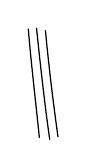
\begin{tikzpicture}[x=1mm,y=1mm,line width=.45pt,line cap=round]
\draw (0,14.0) .. controls (.36,9.6) and (1.02,4.1) .. (1.40,.25);
\draw (1.05,14.1) .. controls (1.53,9.4) and (2.14,4.0) .. (2.72,0);
\draw (2.18,13.8) .. controls (2.62,9.0) and (3.26,4.0) .. (3.77,.32);
\end{tikzpicture}}}
\margin{\uline{N.B.} \unsure{if|If} $u,\sigma$ are elements of a group $G$, one of course sets $u(\sigma)=u\sigma u^{-1}$.}
\margin{this \uline{implies that}, \deleted{\unsure{by}} $\operatorname{int}(u_{\alpha,\beta,f})$ has the same effect, \unsure{on|in} $\mathrm{Sl}(2,\widehat{\mathbb Z})'$ as the \unsure{automorphism} $u$ of $\unsure{\widehat{\mathcal G}_{0,3}^{+}|\widetilde{\mathcal G}_{0,3}^{\to}}$ defined (when there is one), by passage to the quotient in $\mathrm{Sl}(2,\widehat{\mathbb Z})'$.}

formulas which reduce to formulas in which $f$ has again disappeared
\[
(81)\qquad
\left\{\begin{aligned}
u_{\alpha,\beta}(\sigma_\infty)&=\operatorname{int}(\beta)(\sigma_\infty)\\
u_{\alpha,\beta}(\rho)&=\operatorname{int}(\unsure{\alpha|\beta})(\rho)
\end{aligned}\right.,
\]
which \deleted{in turn} follow \inserted{\uline{trivially}} from the two expressions \deleted{of} (78) for $u_{\alpha,\beta}$!

The formulas (80) are naturally completed by
\[
(82)\qquad
u_{\alpha,\beta,f}(\varepsilon_0)
=\deleted{\unsure{f\varepsilon_0}}\inserted{\varepsilon}\operatorname{int}(f^{-1})(\varepsilon_0^\mu)
\qquad\deleted{\unsure{(\varepsilon=\varepsilon_2)}}
\]
\[
(\text{where }\varepsilon=\varepsilon_2\in\{\pm1\})
\]
\margin{\figure{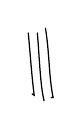
\begin{tikzpicture}[x=1mm,y=1mm,line width=.45pt,line cap=round]
\draw (0,8.6) .. controls (.28,5.5) and (.48,2.7) .. (.75,.7) -- (.48,.86);
\draw (1.15,8.6) .. controls (1.44,5.1) and (1.52,2.0) .. (2.0,0);
\draw (2.18,9.2) .. controls (2.68,6.2) and (2.62,2.9) .. (3.15,.43) -- (2.90,.39);
\end{tikzpicture}}}
which in turn reduces to
\[
(83)\qquad u_{\alpha,\beta}(\varepsilon_0)=\varepsilon.\varepsilon_0^\mu
\]
where $f$ no longer appears. Since $\varepsilon_0=\sigma_\infty\rho$, this formula reduces to:
\[
u_{\alpha,\beta}(\sigma_\infty)u_{\alpha,\beta}(\rho)=\varepsilon.\varepsilon_0^\mu,
\]
which in view of (81) reduces to:
\[
\operatorname{int}(\beta)(\sigma_\infty)\operatorname{int}(\unsure{\alpha|\beta})(\rho)=\varepsilon.\varepsilon_0^\mu
\]
\deleted{\unsure{then}}
\[
\deleted{\unsure{\alpha\sigma_\infty\alpha^{-1}\beta\rho\beta^{-1}}}
\]

\scanpage{201}

now the first \unsure{side} is written
\[
\deleted{\unsure{\beta\sigma_\infty\beta^{-1}\alpha\rho\alpha^{-1}
=(\beta\sigma_\infty\beta^{-1}\sigma_\infty)(\sigma_\infty\rho)(\rho^{-1}\alpha\rho\alpha^{-1})}}
\]
\[
\deleted{\unsure{=(\beta\sigma_\infty(\beta)^{-1})\varepsilon_0(\rho^{-1}(\alpha)\beta^{-1})}}
\]
\[
\begin{aligned}
\beta\sigma_\infty\beta^{-1}\alpha\rho\alpha^{-1}
&=\underbrace{(\beta\sigma_\infty\beta^{-1}\sigma_\infty)}_{\beta\sigma_\infty(\beta)^{-1}}
\underbrace{(\sigma_\infty\rho)}_{\varepsilon_0}
\underbrace{(\rho^{-1}\alpha\rho\alpha^{-1})}_{\rho^{-1}(\alpha)\alpha^{-1}=\rho^{-1}(\alpha\rho(\alpha)^{-1})}\\
&=\eta.\varepsilon_0.\rho^{-1}(\xi)
=\eta.\underbrace{(\varepsilon_0\rho^{-1})}_{\sigma_\infty}(\xi).\varepsilon_0
=\eta\sigma_\infty(\xi)\varepsilon_0
\end{aligned}
\]
so relation (83) is also written
\[
\eta\sigma_\infty(\xi)=\varepsilon\varepsilon_0^{\mu-1}\quad(=\varepsilon \ell_0^\nu)
\]
now one has $\xi=\varepsilon\eta \ell_1^\nu$ (loop relation (60))

so
\[
\eta\sigma_\infty(\xi)=\varepsilon\eta\sigma_\infty(\eta)\ell_0^\nu=\varepsilon \ell_0^\nu,\quad\text{OK.}
\]

\uline{Remark.} All these formulas are valid in $\mathrm{Gl}(2,\widehat{\mathbb Z})$, without ambiguity of signs, once $\alpha,\beta,f$ are chosen. If one changes the signs of $\alpha$ \unsure{or|and} of $\beta$ or both, the loop relation is not modified --- and $u_{\alpha,\beta}$ is not \unsure{changed} either, \deleted{On the other hand} nor $u_{\alpha,\beta,f}$ (if one does not touch $f$). On the other hand, a \unsure{change} of sign on $f$ implies a \unsure{change} of sign on $u_{\alpha,\beta,f}$. But such a change of sign of course changes nothing as to the validity of formulas (80), (82). When one makes

\scanpage{202}
\mspage{400}

on $(\alpha,\beta,f)$ the changes \unsure{the}
\[
(84)\qquad
\alpha'=\ell_0^n\alpha,\qquad\beta'=\ell_0^n\beta,\qquad f'=\ell_0^n f
\qquad(n\in\mathbb Z)
\]
then \deleted{\illegible{1}}
\[
(85)\qquad
\left\{\begin{aligned}
c'&=\unsure{c},\quad d'=d& t'&=t,\quad u'=u\\
\underbrace{f'^{-1}\alpha'}_{\alpha'_0}&=\underbrace{f^{-1}\alpha}_{\alpha_0}&
\underbrace{f'^{-1}\beta'}_{\beta'_0}&=\underbrace{f^{-1}\beta}_{\beta_0}
\end{aligned}\right.
\qquad\deleted{\unsure{\mu'=\mu|u'=u}}
\]
\deleted{finally}
\[
\deleted{\unsure{\delta'=\delta}\text{ since}}
\qquad\deleted{\unsure{u_{\alpha',\beta'}}}
\]
finally
\[
\delta'(=\det\alpha')=\delta(=\det\alpha)\quad(\text{since }\det \ell_0^n=1)
\]
\[
(86)\qquad
\left\{\begin{aligned}
\text{hence}\quad\deleted{\unsure{f}}\quad
\mu'\bigl(=\delta'/(c'^2+c'd'+d'^2)\bigr)&=\mu\bigl(=\delta/(c^2+cd+d^2)\bigr)\\
\text{hence}\quad\varepsilon'_2&=\varepsilon_2,\quad\alpha'_2=\alpha_2.
\end{aligned}\right.
\]
this is \unsure{twice} what is needed to check \inserted{with (79)} that
\[
(87)\qquad u_{\alpha',\beta',f'}=u_{\alpha,\beta,f}.
\]

Let us also recall (cf. proposition page 384)

\uline{Proposition.} Let $\mu\in\widehat{\mathbb Z}^*$, hence the signs $\varepsilon_2=\varepsilon_2(\mu)$ and $\varepsilon_3=\varepsilon_3(\mu)$ (defined by $\mu\equiv\varepsilon_2\ (4)$, $\mu\equiv\varepsilon_3\ (3)$), and let $c,d,t,u\in\widehat{\mathbb Z}$. For there to exist $a,b,r,s\in\widehat{\mathbb Z}$
\[
\alpha=\begin{pmatrix}a&b\\c&d\end{pmatrix},\qquad
\beta=\begin{pmatrix}r&s\\t&u\end{pmatrix}
\quad\text{satisfying (64)}
\]
\[
ad-bc=\varepsilon_3\qquad ru-st=1
\]
and the loop relation
\[
\alpha\rho(\alpha)^{-1}=\varepsilon_2\bigl(\beta\sigma_\infty(\beta^{-1})\bigr)\ell_1^\nu
\qquad\text{where }\nu=(\mu-1)/2
\]
(i.e. relations (73)) it is necessary and sufficient that one have
\[
(88)\qquad\varepsilon_3(c^2+cd+d^2)=\varepsilon_2(t^2+u^2)=1/\mu,
\]
and \unsure{the set|the set} of pairs $(\alpha,\beta)$ satisfying these conditions is a \uline{torsor} under $\widehat{\mathbb Z}$, operating

\margin{\uline{N.B.} For fixed $\mu$, one can always find $c,d,t,u$ satisfying relation (88) --- fortunately!}

\scanpage{203}

by
\[
 (\alpha,\beta)\longmapsto
 (\unsure{\varepsilon_0^n}\alpha,\varepsilon_0^n\beta).
\]
\deleted{\illegible{1}}

\uline{Corollary} For one to be able to find $\alpha,\beta$ such that one has in addition $\alpha\equiv\beta\equiv1\ (2)$, it is necessary and sufficient that one have
\[
\tag{89}
 c\equiv t\equiv0\ (2)\qquad d\equiv u\equiv\unsure{1}\ (2),
\]
and then \unsure{the set} of solutions $(\alpha,\beta)$ satisfying these additional conditions is a torsor under $\widehat{\mathbb Z}$, operating by
\[
 (\alpha,\beta)\longmapsto(\ell_0^n\alpha,\ell_0^n\beta).
\]

\uline{Scholium} One can thus say that for an element \inserted{$u$} of $\mathcal N_{0,3}^{!\sim}$, which defines \unsure{thus|two} $\alpha,\beta$ in $\Pi_{0,3}^{\sim\wedge},\Pi_{0,3}^{\wedge}$ \inserted{(\uline{modulo} the \unsure{transformations} $(\alpha,\beta)\mapsto(\ell_0^n\alpha,\ell_0^n\beta)$),} (satisfying the loop relation), there are attached to it the ``adelic invariants'' \deleted{\illegible{3}}
\[
\tag{90}
 \Theta=(\mu,c,d,t,u)
\]
($c,d,t,u$ determined up to \unsure{\uline{ambiguities}|ambiguities} of sign, and no more) satisfying (88) --- and this is \uline{the best one can do} in the present context: the $a,b,r,s$ \unsure{have|is} not an invariant character. When one has an element \inserted{$\underline u$} of $\unsure{\mathcal M_{0,3}^{!\sim}|\mathcal N_{0,3}^{!\sim}}$ --- i.e. an \unsure{actual} automorphism, not just outer --- one has in addition an $\underline f\in\Pi_{0,3}^{\wedge}$, giving an $f\in\mathrm{Sl}(2,\widehat{\mathbb Z})'$, whence
\[
\tag{91}
 f=\begin{pmatrix}\unsure{j}&\unsure{k}\\ \ell&m\end{pmatrix}
 \qquad\begin{gathered}\uline{\text{defined modulo signs}}\\
 \text{and modulo } f\longmapsto\ell_0^n f
 \end{gathered}
\]

\scanpage{204}
\mspage{401}

\deleted{whence \unsure{thus} one}

But this additional datum is a little too
\deleted{$u_{\alpha,\beta,f}=u_{\mu,c,d,t,u}$}
weak to reconstruct \deleted{$u_{\alpha,\beta,f}$} the element
\[
 \uuline{u}\inserted{{}=\varphi(\underline u)}\deleted{\unsure{\mathrm{d\acute{e}f}}}
 =u_{\alpha,\beta,f}
\]
of $\mathrm{Gl}(2,\widehat{\mathbb Z})'$ associated to $u$.

It is better to say that for fixed $\mu,c,d,t,u$ one has a $\widehat{\mathbb Z}$-torsor of $(\alpha,\beta)\equiv(1,1)\ (2)$ satisfying the conditions stated \unsure{in|of} the proposition \unsure{§|,} and its corollary, let $T=T_\Theta$, one then makes $\widehat{\mathbb Z}$ operate \unsure{diagonally} on $T\times\mathrm{Sl}(2,\widehat{\mathbb Z})$ by
\[
 (\alpha,\beta,f)\longmapsto
 (\ell_0^n\alpha,\ell_0^n\beta,\ell_0^n f)
\]
and one looks at the quotient --- this is thus the twist by $\check T$ (torsor opposite to $T$) of $\mathrm{Sl}(2,\widehat{\mathbb Z})$, on which $\widehat{\mathbb Z}$ operates by $f\longmapsto\ell_0^n f$. \deleted{One must} it is the datum of an element \inserted{$f$} of
\[
 \check T_\Theta\unsure{\mathbin{\wedge}_{\widehat{\mathbb Z}}}\mathrm{Sl}(2,\widehat{\mathbb Z})
 \deleted{\unsure{=\mathcal G_\Theta}}
\]
\margin{it is an $\mathrm{Sl}(2,\widehat{\mathbb Z})$-torsor on the \uuline{right}}
which makes it possible to define an element
\[
 \uuline{u}=u_{\alpha,\beta,f},
\]
which changes sign if $f$ is replaced by $(f(-1))$.

Decidedly, these formulations are not exciting, and it is becoming clear that it will be necessary to introduce explicit-

\scanpage{205}

ly and study \deleted{in a manner}\inserted{\unsure{with}} a minimum of care the \uline{adelic group} formed by the systems $(\alpha,\beta,f)$ satisfying the loop relation, and \deleted{\unsure{consider}} the canonical homomorphism from $\mathcal M_{0,3}^{!\sim}$ into the said group.

But I would like before that to finish the notational scales.

\deleted{\illegible{1}}

\scanpage{206}
\mspage{402}

\uline{$\overline{\mathrm{IV}}$} The three fundamental special cases.

We return to the elements $g,h,f$ etc. \uline{in} $\Pi_{0,3}^{\wedge}$ and $\Pi_{0,3}^{\sim\wedge}$ which correspond to $u$, which can be \unsure{described|described} in four different ways, by one or another of the four systems
\[
\tag{92}
 (g,h,f),\quad(\alpha_0,\beta_0,f),\quad(\alpha,\beta,f),\quad(\xi,\eta,f).
\]

\inserted{\unsure{$1^\circ$|$1^{\mathrm{er}}$}\ \uline{Case}:}
\deleted{\illegible{1}\ \uline{Case}\ \illegible{1}}
\[
\tag{93}
 h=1,\quad\text{i.e. }\beta_0=1,\quad\text{i.e. }\beta=f,\quad
 \text{i.e. }\eta=f\sigma_\infty(f)^{-1},
\]
i.e.
\[
\tag{94}
 [u,\sigma_\infty]=1.
\]

For a $u$ \inserted{\uline{whatsoever}} \unsure{(}i.e. an arbitrary system $(g,h,f)$ etc., there is one and only one inner \unsure{automorphism} $\operatorname{int}(\gamma)$ such that \inserted{$u'=\operatorname{int}(\gamma)\unsure{u}$} \unsure{satisfies} the preceding property i.e. commutes with $\sigma_\infty$, \deleted{\illegible{1}} this will be for
\[
 \gamma=\beta_0^{-1}\qquad(\text{cf. formulas (49)}).
\]
\deleted{\illegible{1}}

The $u$ satisfying (93), expressed in terms of triples $(\xi,\eta,f)$ satisfying the three relations (44) (46) (not involving $f$), \deleted{\illegible{1}} thus correspond (by the relation $\eta=f\sigma_\infty(f)^{-1}$ of (93)) to the \deleted{\unsure{triples}} pairs $(\xi,f)$ of elements of $\Pi_{0,3}^{\wedge}$, satisfying
\[
\tag{95}
 \xi\,\rho(\xi)\,\rho^2(\xi)=1
\]
\[
\tag{96}
 \xi=(f\sigma_\infty(f)^{-1})\ell_1^\nu
\]
\inserted{with $\nu\in\widehat{\mathbb Z}$, as a \unsure{variable}, such that $2\nu+1\in\widehat{\mathbb Z}^{*}$}

\margin{\uline{N.B.} \unsure{one will have}
$\xi=fg\rho(f)^{-1}$.
\unsure{in place of} $f$ \unsure{it is permissible|it is legitimate} \unsure{to write} \unsure{here} $\unsure{\beta}$ --- \unsure{but then} \illegible{2} $\unsure{\beta}$ \unsure{determined} \unsure{by} \illegible{2} $\unsure{\ell_0^n}$ \illegible{2} $\unsure{f\longmapsto\ell_0^n f}$ \illegible{2}}
